
\subsection{B. Analysis of the energy consumption structure evolution}
\subsubsection{Introduction of information entropy}
Energy consumption structure of different areas are always quite different because of different energy storage situation and economic level. Therefore, it's hard to adopt a specific index the quantify the structure evolution. As Hollis B. Chenery said, economic development is accompanied by the structural transformation. This structural transformation is mainly embodied in the next two aspects: the industrial structure upgradation and energy consumption structure evolution. As the economic development, cleaner and higher-efficiency energy will replace the traditional and lower-efficiency energy. Commonly, also as figures of the four states' energy profile shows, the natural gas, nuclear energy and renewable energy take higher proportion.

Here we utilize the concept of \textit{information entropy} to quantificationally describe the energy consumption evolution. Entropy is a state function to describe the irreversibility of spontaneous process, defined based on the second law of thermodynamics \cite{gibbs1906scientific}. Boltzmann gave the following entropy function:
\begin{equation}
    S = K_B \ln{P}
\end{equation}
where $K_B$ is Boltzmann constant, $P$ is the probability that the system is in a certain state. In 1908, Shannon introduced the concept of entropy to the information theory and defined it as information entropy $\mathrm {H}$:
\begin{equation}
     H(X)= E [I(X)]= E [-\ln(P(X))]
    \label{equa: Shannon}
\end{equation}
where $E$ is the expected value operator, and $ {I}$ is the information content of $X$. $ {I}(X)$ is itself a random variable \cite{borda2011fundamentals}. The equation above is called Shannon Equation, it can describe the degree of randomness and disorder of any system or material \cite{Cai1998}.

Follow what Shannon has done, we introduce the information entropy to the energy consumption structure analysis. The energy consumption system is a non-linear open system that has wide material, energy and information exchange with the environment. As time passes, it's structure shows a spontaneous and irreversible evolution, this satisfies the consumption of dissipative structure system. For example, consider an energy consumption structure with $m$ types of energy (the unit must be uniform), and the quantity of $i$th energy is ${H}_i$, thus is proportion is ${P}_i={H}_i/\sum{H_i}=H_i/H$. Therefore, the information entropy of energy consumption structure is:
\begin{equation}
    S = -\sum_{i=1}^m{P_i \ln{P_i}}
    \label{equa: ie of E}
\end{equation}
Particularly, when there is only one type of energy in the system, $S_{\mathrm{min}}=0$; on the contrary, when all the energy types are equal, then $H_1=H_2=\dots=H_m=H/m$, then $S_{\mathrm{max}}=\ln{m}$. In the real world, such two extreme situation will never appear, thus information entropy is between $S_{\mathrm{min}}$ and $S_{\mathrm{max}}$, and it can reflects the complexity of the energy concumption structure.

Further more, we can define the equilibrium and dominance degree. Based on the information entropy equation, the equilibrium degree can be given by:
\begin{equation}
    E=-\sum_{i=1}^m{P_i \ln{P_i}}/\ln{m}
    =S/\ln{m}
\end{equation}
i.e., the equilibrium degree is the ratio of information entropy to the maximum entropy. Larger $E$, smaller difference of the proportion of different types of energy. The dominance degree is $D=1-E$, and it reflects the support ability of one or several types of energy to the energy consumption, which is the contrast to the equilibrium degree. 

\subsubsection{Summary of information entropy }
Time series of the $S$, $E$ and $D$ of four states are calculated and can be seen from figure \ref{fig: SED}. It should be emphasized that due to the existence of negative values in ELISB (net interstate sales of electricity and associated losses), it is ignored when calculate the information entropy. In this figure, the information entropy of the four states has a trend of continuously increasing by time. This means the degree diversification and complexity of them are increasing, which may be a result of economic development. Besides, the equilibrium degree always increases and the dominance equilibrium degree always decrease by time, which can also suggest that the energy consumption structure is more balanced. 

Combine figure \ref{fig: prop} and \ref{fig: SED}, we can see in  the four states, the Arizona state is most diversified, with largest proportion of nuclear energy. New Mexico state also has larger information entropy as it has a balanced structure of coal, petroleum and natural gas. California and Texas shows similar diversity, their the proportion of natural gas and petroleum is similar but California consume more renewable and nuclear energy and Texas consume more coal. 
\begin{figure}[H] 
    \centering 
    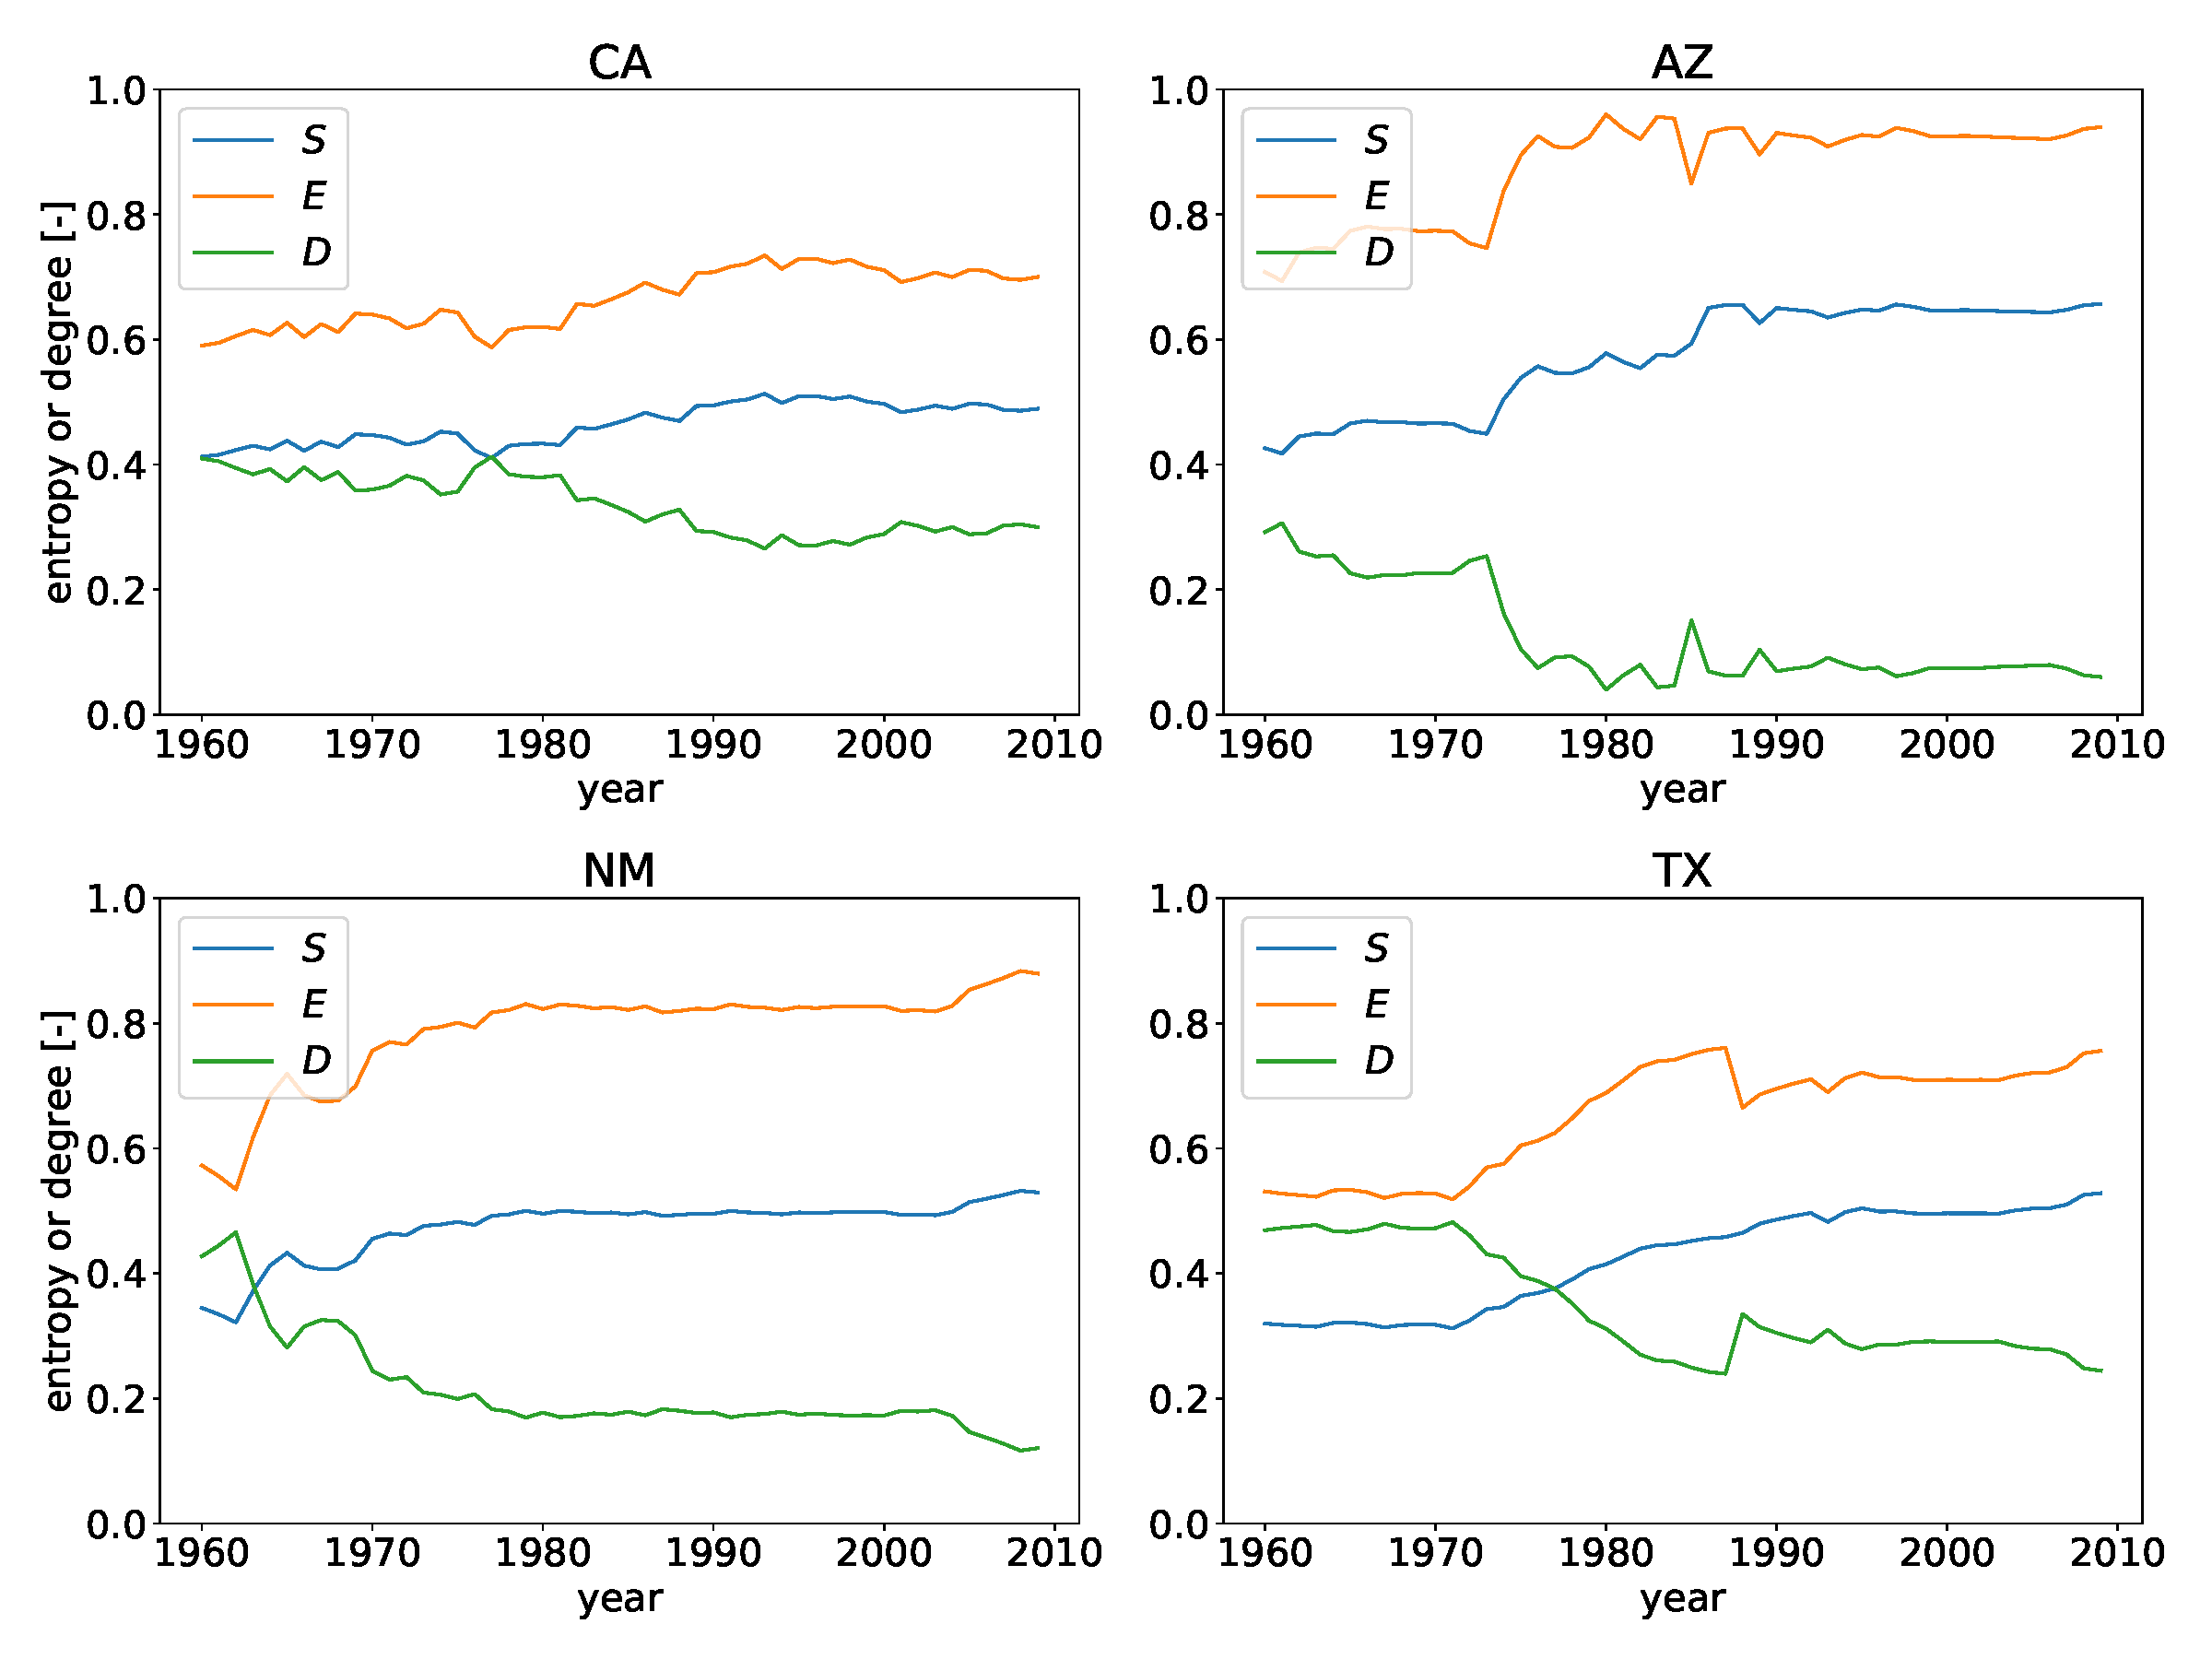
\includegraphics[width=0.6\linewidth]{fig/entropy.pdf}
    \caption{Information entropy $S$, equilibrium degree $E$ and dominance degree $D$ of four sates from 1960 to 2009}
    \label{fig: SED}
\end{figure}

\subsubsection{Regression analysis of energy consumption evolution}
Here we need to find the factors in the data-set that are relevant to the energy consumption.
\begin{enumerate}
    \item{Relevant factors}\par
The factors we apply are divided into the next classes:
\begin{enumerate}
    \item{Geographic factors}
    \par
    These factors are mainly the energy possessed by the region, such as coal, hydroenergy, natural gas, crude oil, related factors in the data-set are:
    \begin{itemize}
        \item CLPRB (coal production)
        \item HYTCB (hydroelectricity total production)
        \item NGMPB (natural gas marketed production),
        \item PAPRB (crude oil production (including lease condensate))
    \end{itemize}

    \item{Industrial factors}
    \par
    The energy consumed by different sectors can reflect the their volume. According to the third and forth alphabet of the MSNCODE, we select the total energy (TE) of:
    \begin{itemize}
    \item{AC} transportation sector consumption, MSNCODE=TEACB
    \item{CC} commercial sector consumption, MSNCODE=TECCB
    \item{EG} electric power sector generation (also generation), MSNCODE=TEEGB
    \item{EI} electric power sector consumption, MSNCODE=TEEIB
    \item{IC} industrial sector consumption, MSNCODE=TEICB
    \item{RC} residential sector consumption, MSNCODE=TERCB
    \end{itemize}
    \item{Economic factors}
    \par
    As discussed above, the economic development means the structural transformation, which includes the energy consumption structure evolution. Economic factors include GDP (MSNCODE=GDPRX), GDP growth rate (calculated from GDP: $\mathrm{GR}_i=\frac{\mathrm{GDP}_{i+1}-\mathrm{GDP}_{i}}{\mathrm{GDP}_{i}}$) and total energy consumption per real dollar of GDP (MSNCODE=TETGR). It might also be noted that 
    GDP data starts from 1977, and years before that GDP and it's growth rate is treated as zero.
    
    In adtion, the average prices of different types of energy are also considered. These include:
    \begin{itemize}
        \item CLTCD (coal average price, all sectors)
        \item NGTCD (natural gas average price, all sectors (including supplemental gaseous fuels)
        \item PATCD (all petroleum products average price, all sectors)
        \item NUETD (nuclear fuel average price, all sectors)
        \item ESTCD (electricity average price, all sectors). 
        \item Renewable energy average price, all sectors (with similar MSNCODE RETCD). This is not supplied in the data-set, and is calculated by the following equation:
        \begin{equation}
            \mathrm{RETCD} = \frac{\mathrm{TETCV}-\sum{\mathrm{XTCB}\cdot \mathrm{XTCD}}}
                {\mathrm{RE}}
        \end{equation}
        where $\mathrm{X}$ can be CL, NG, PA or NU, and TETCV is total energy expenditures.
        
    \end{itemize}
    \item{Demographic factors}
    \par
    Population of the a state may affect the amount of the energy consumption if the difference of that of the individuals is not too large. MSNCODE here is TPOPP (resident population including armed forces).
    \item{Climate factors}
    \par
    Climate influence the energy consumption by influencing people's behaviour. For example, the temperature. When it gets hotter, the air conditioning may run; when it becomes colder, the heating may work. As another example, the precipitation. When the state suffer drought, pumps may launch; when the state meet flood, life and production activities may be impeded and energy consumption may be reduced. NCEI (National Centers For Environmental Information) has collected climate and weather datasets (\url{https://www.ncdc.noaa.gov}). We adopt annually averaged temperature and precipitation from four stations in four states from “U.S. Local Climatological Data”, including station Tucson for Arizona, station Bakersfield for California, station Albuquerque for New Mexico, station Abilene for Texas.
\end{enumerate}

\item{Multiple linear regression model}\par
The data set here is $\{{y_{i},x_{i1},\ldots ,x_{ip}\}}_{i=1}^{n}$ of $n$ years ($n$=50 and $p$=23, i.e., number of the indices). The linear regression assume the relationship between the development variable $y_i$ and the $p$-vector of regressors $x_i$ is linear.
Before establishing the regression model, all the data should be normalize. The normalized variable $x_{i}'$ is given by:
\begin{equation}
    x_{i}' = \frac{x_{i}-\bar{x_{i}}}{std(x_i)}
\end{equation}
The normalization treatment can prevent the larger variable from hiding the influence of smaller variable.

The multiple linear regression model takes the form:

\begin{equation}
    y_i = \beta_0 1 + \beta_1 x_{i1} + \beta_2 x_{i2} + \cdots + \beta_n x_{ip}+\varepsilon_i=\mathbf{x}_i^{\top}\mathbf{\beta} + \varepsilon_i
\end{equation}
where $\beta_i$ is the coefficient, $\varepsilon_i$ is random variable. The vector form of the $n$ equations is:
\begin{equation}
    \mathbf{y}=\mathbf{X} \boldsymbol \beta+\boldsymbol \varepsilon
\end{equation}
where:
\begin{equation*}
    \mathbf {y} =
    {\begin{pmatrix}
    y_{1}\\
    y_{2}\\
    \vdots \\
    y_{n}
    \end{pmatrix}},\quad {\mathbf{X}={
    \begin{pmatrix}
    \mathbf {x} _{1}^{\top }\\
    \mathbf {x} _{2}^{\top }\\
    \vdots \\
    \mathbf {x} _{n}^{\top }
    \end{pmatrix}}
    =
    {\begin{pmatrix}
    1&x_{11}&\cdots &x_{1p}\\
    1&x_{21}&\cdots &x_{2p}\\
    \vdots &\vdots &\ddots &\vdots \\
    1&x_{n1}&\cdots &x_{np}\end{pmatrix}}}
\end{equation*}
\begin{equation*}
    {\displaystyle {\boldsymbol {\beta }}={
    \begin{pmatrix}
    \beta _{0}\\
    \beta _{1}\\
    \beta _{2}\\
    \vdots \\
    \beta _{p}
    \end{pmatrix}},\quad {\boldsymbol {\varepsilon }}=
    {
    \begin{pmatrix}
    \varepsilon _{1}\\
    \varepsilon _{2}\\
    \vdots \\
    \varepsilon _{n}
    \end{pmatrix}}
    }
\end{equation*}

Select a $\boldsymbol{\beta}$'s estimation $\hat{\boldsymbol{\beta}}$ by using the Ordinary Least Squares (OLS) estimator (minimize the sum of the squares of $\boldsymbol{\varepsilon}$), namely:
\begin{equation}
    \min{\sum{\boldsymbol{\varepsilon}^2}} = \min{(\mathbf{Y}-\mathbf{X}\boldsymbol{\beta})^{\top}(\mathbf{Y}-\mathbf{X}\boldsymbol{\beta})}
\end{equation}
The solution of the equation above is:
\begin{equation}
    {\displaystyle {\hat {\boldsymbol {\beta }}}=(\mathbf {X} ^{\top }\mathbf {X} )^{-1}\mathbf {X} ^{\top }\mathbf {y} =\left(\sum \mathbf {x} _{i}\mathbf {x} _{i}^{\top }\right)^{-1}\left(\sum \mathbf {x} _{i}y_{i}\right)}
\end{equation}
Finally, we can get the estimation of the dependent variable:
\begin{equation}
    \hat{\mathbf{Y}} = \mathbf{X}^{\top} \hat{\boldsymbol{\beta}}
\end{equation}

\item{Regression results of energy profile evolution} \par
To characterize the evolution of the energy profile of each of the four states, we first regress information entropy on all the possible factors listed above. Figure \ref{fig: entropy regress} shows the real and the estimated data. All the $R^2$ reach 0.96, suggest that the information entropy is strongly linear correlated to the factors. Take Arizona for example, the regression overview in Stata is shown in figure \ref{fig: entropy stata}.
\begin{itemize}
    \item $P$ value of the $F$ test is 0.0000, shows a highly significant relativity for regression equation.
    \item Generally, if the $P$ value of the $t$ test of a variable is smaller than 0.05 (with a confidence level of 95\%), we can refuse the hypothesis that the variable is not related to the dependent variable. These include: CLPRB, HYTCB, NGMPB, NUETD, RETCD, TPOPP, TEEIB, TERCB. 
    \item Since all the factors has been normalized, their coefficients can reflect their contribution rate to the dependent variable. Top 3 variables of that are TERCB (0.206), TEEIB (0.194), TPOPP (0.166), that's say, the information entropy (the diversity or complexity of the energy profile) has a strong positive correlation with total energy consumed by the residential, total energy consumed by the electric power sector and residential population. This is an evidence of the economic development influences the energy profile. 
\end{itemize}
\begin{figure}[H] 
    \centering 
    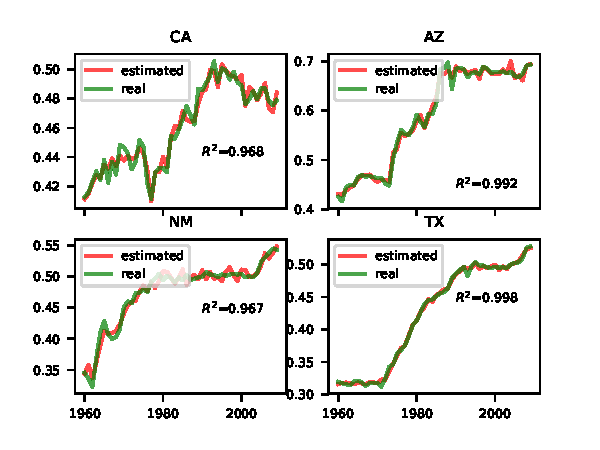
\includegraphics[width=0.6\linewidth]{fig/entropy_estimation.pdf}
    \caption{The real and estimated information entropy of the four states from 1960 to 2009}
    \label{fig: entropy regress}
\end{figure}

\begin{figure}[H] 
    \centering 
    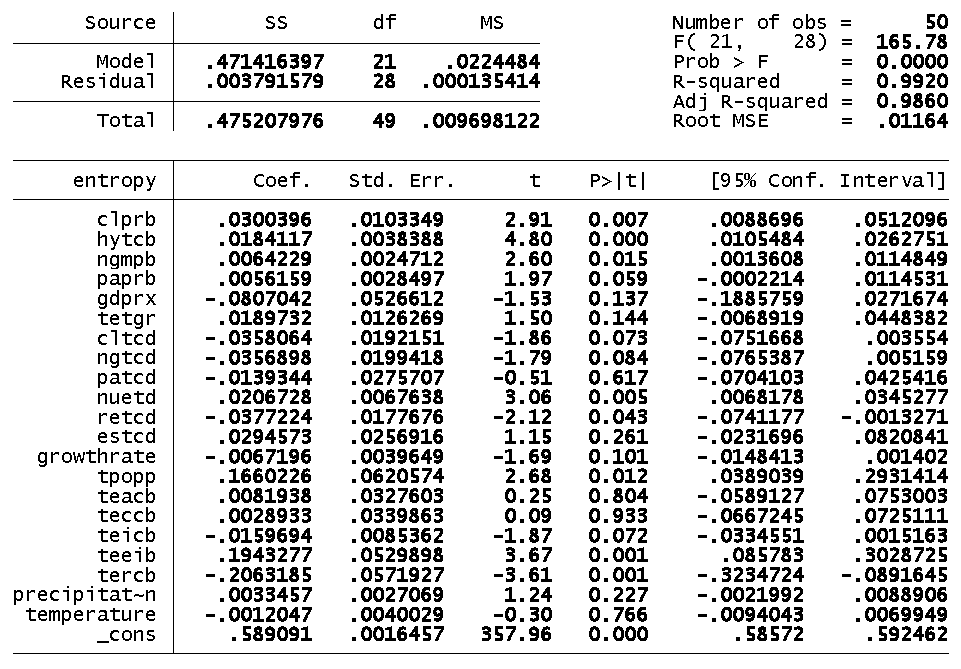
\includegraphics[width=0.6\linewidth]{fig/entropy_AZ.pdf}
    \caption{Overview of the regression of information entropy on all the listed factors of Arizona in Stata}
    \label{fig: entropy stata}
\end{figure}

\item{Regression results of consumption of renewable energy}\par
Figure \ref{fig: RE regress} shows the real and the estimated renewable energy.  All the $R^2$ reach 0.96, suggest that the information entropy is strongly linear correlated to the factors. Take Arizona for example, the regression overview in Stata is shown in figure \ref{fig: RE stata}.
\begin{itemize}
    \item $P$ value of the $F$ test is 0.0000, shows a highly significant relativity for regression equation.
    \item Significant variables include: HYTCB, PATCD, TEACB, TEEIB, and they all have relatively larger coefficient. Hydroelectricity belongs to renewable energy and is also connected to geographic features. If it plays an important role in renewable energy, it's not surprise that it's coefficient is large. Price of petroleum also positively influence RE, as petroleum is one of the substitute of RE. Total energy consumed by transportation sector and electric power sector both negatively influence RE. However, when we regress RE on these four variables, coefficient of TEEIB turns to be positive. A possible explanation is that several variable in the list is negative relevant to TEEIB and positive relevant to RE.   
\end{itemize}
\begin{figure}[H] 
    \centering 
    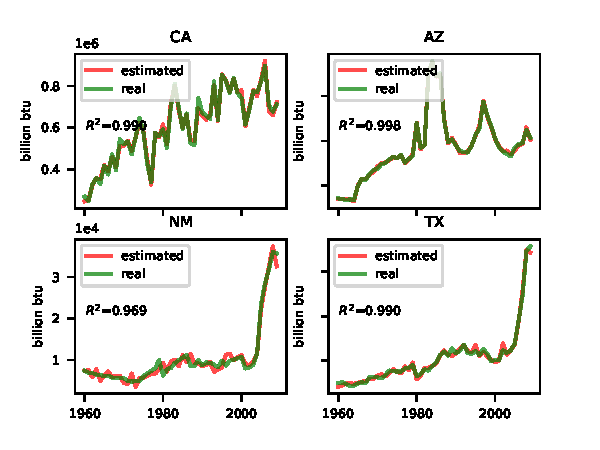
\includegraphics[width=0.6\linewidth]{fig/RE_estimation.pdf}
    \caption{The real and estimated renewable energy of the four states from 1960 to 2009}
    \label{fig: RE regress}
\end{figure}

\begin{figure}[H] 
    \centering 
    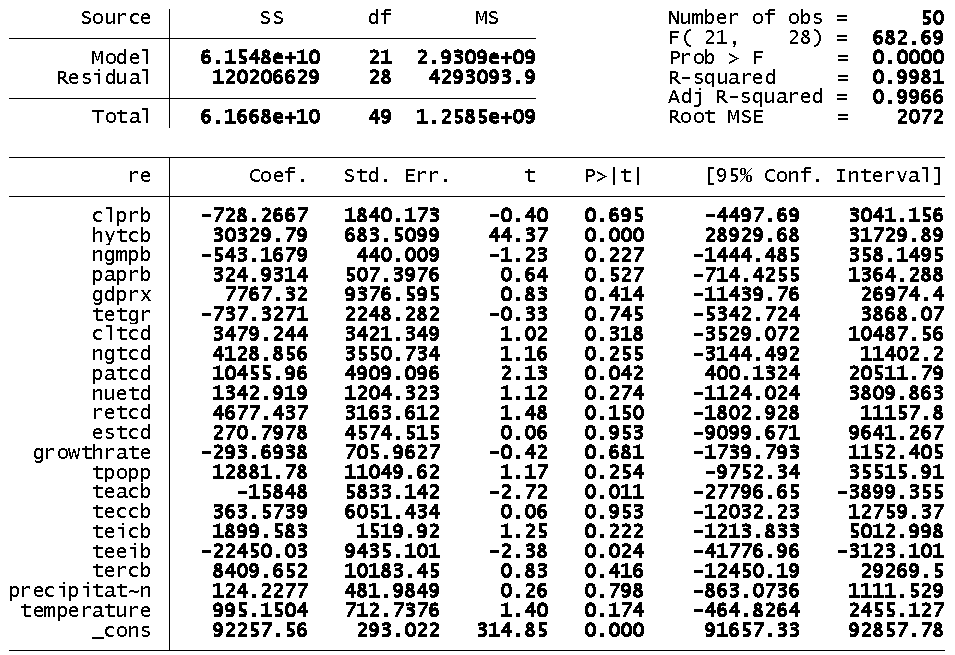
\includegraphics[width=0.6\linewidth]{fig/RE_AZ.pdf}
    \caption{Overview of the regression of renewable energy on all the listed factors of Arizona in Stata}
    \label{fig: RE stata}
\end{figure}

\item{Summary of B}

We summerize all the variables and coefficients with $P<0.05$ of the four states in table 2. Followings are our annalysis:
\begin{itemize}
\item Price of petroleum influences positively RE of California, Arizona, New Mexico and Texas at the same time. As the main energy of four states, growth of petroleum price makes the demand of petroleum decrease, so the amount of RE will grow as RE is the substitute goods of petroleum.
\item In California and Arizona, HYTCB is also an important influencing factors. Hydroelectricity belongs to renewable energy and is also connected to geographic features. If it plays an important role in renewable energy, it’s not surprise that it’s coefficient is large.
\item In California and Texas, population is a main influencing factors because the population of California and Texas is large. The more energy will be demanded with the larger of population, therefore the coefficient of TPOPP is large. 

\item In New Mexico and Texas, CLPRB is a main important influencing factors and the CLPRB influence negatively RE. When coal production becomes large, the price of coal will decline and people are more willing to use coal, which results in the decreasing of RE. 
\item What’s more, the price of renewable energy (RETCD) is significant in New Mexico and Texas. It is obvious that people won’t use renewable energy with high price. As the same reason, the amount of RE will increase when the price of coal is going to be higher in Texas.
\item Specially in Arizona, total energy consumed by the transportation sector (TEACB) and total energy consumed by the electric power sector (TEEIB) both negatively influence RE. However, when we regress RE on these four variables, coefficient of TEEIB turns to be positive. A possible explanation is that several variable in the list is negative relevant to TEEIB and positive relevant to RE.

\end{itemize}
 
 



\begin{table}[H]
\centering

\caption{Variables and their coefficients whose $P<0.05$ of the four states}
\label{table: var and coef}
    \begin{threeparttable}
        \begin{tabular}{cccccccc}
        \toprule
\multicolumn{2}{c}{CA} & \multicolumn{2}{c}{AZ} & \multicolumn{2}{c}{NM} & \multicolumn{2}{c}{TX} \\
\midrule
variable & coef.     & variable & coef.     & variable & coef.     & variable & coef      \\
HYTCB    & 66649.39  & HYTCB    & 30329.79  & CLPRB    & -6233.096 & CLPRB    & -30335.52 \\
GDPRX    & -113341.8 & PATCD    & 10455.96  & PATCD    & 7464.639  & CLTCD    & 34015.41  \\
TETGR    & 37955.93  & TEACB    & -15848    & RETCD    & 3200.461  & PATCD    & 65595.21  \\
PATCD    & 104757.7  & TEEIB    & -22450.03 & TERCB    & 8226.356  & RECTD    & 43622.03  \\
TPOPP    & 210763    &          &           &          &           & ESTCD    & -45093.49 \\
         &           &          &           &          &           & TPOPP    & 119151.5   \\
         \bottomrule
\end{tabular}
    \end{threeparttable}
    
\end{table}
\end{enumerate}